%%%%%%%%%%%%%%%%%%%%%%%%%%%%%%%%%%%%%%%
% PlushCV - Cover Letter Template
% Passend zum One Page Two Column Resume
%
% IMPORTANT: THIS TEMPLATE NEEDS TO BE COMPILED WITH XeLaTeX
%
%%%%%%%%%%%%%%%%%%%%%%%%%%%%%%%%%%%%%%

\documentclass[]{plushcv}
\usepackage[ngerman]{babel} % <--- Sorgt für das deutsche Datumsformat bei \today
\usepackage{fancyhdr}
\usepackage{tikz} 
\pagestyle{fancy}
\fancyhf{}

\begin{document}
	
	% =========================================================
	% HAUPTFARBE HIER ÄNDERN (Muss zwingend nach \begin{document} stehen!)
		% =========================================================
		\definecolor{primary}{RGB}{242, 142, 7}  %Firmenfarbe
		% --- DER NEUE FIX FÜR DEN FEHLER ---
		\colorlet{PRIMARY}{primary} % Fängt ab, wenn das Template den Text großschreibt!
		% -----------------------------------
		
		% Diese Befehle zwingen die Vorlagen-Variablen auf deine Farbe:
		\colorlet{headings}{gray}
		\colorlet{subheadings}{black}
		% =========================================================
		
		% --- PORTRAIT FOTO --- 
		% Im Anschreiben oft weggelassen, aber hier der Vollständigkeit halber (auskommentiert)
		% \begin{tikzpicture}[remember picture,overlay]
			%     \node[anchor=north east, inner sep=0pt, xshift=-0.5cm, yshift=-0.5cm] at (current page.north east) {
				%         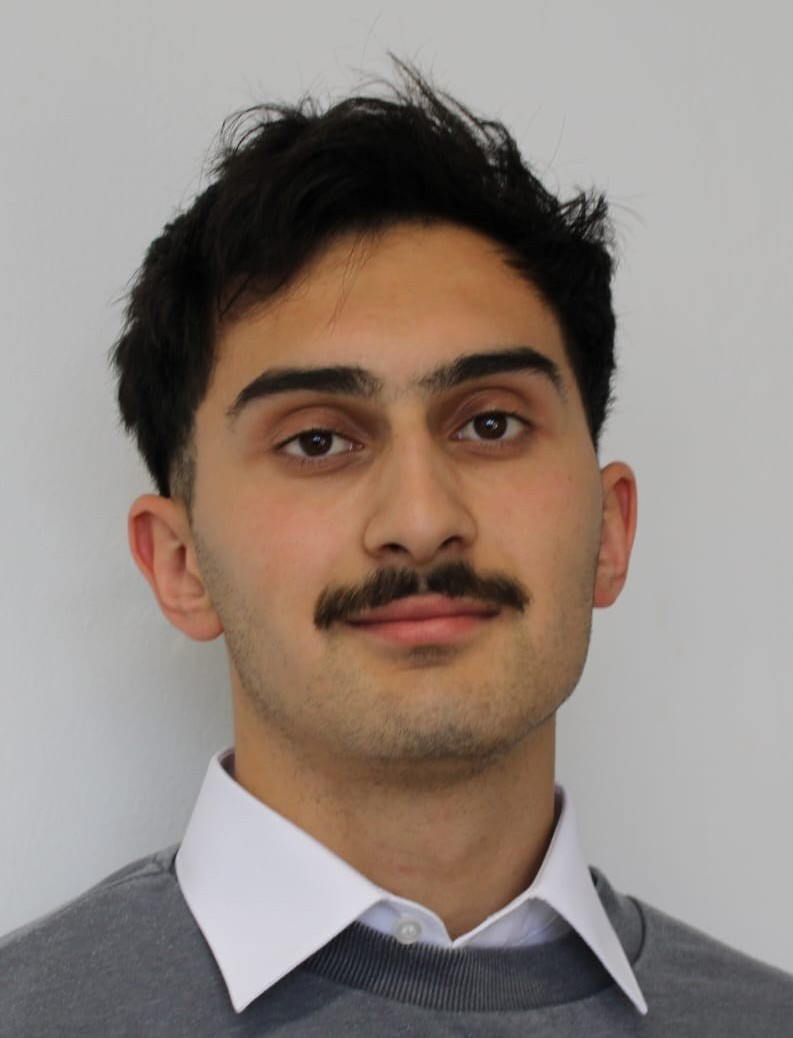
\includegraphics[height=4.5cm]{foto.jpeg}
				%     };
			% \end{tikzpicture}
		% ---------------------
		
		%%%%%%%%%%%%%%%%%%%%%%%%%%%%%%%%%%%%%%
		%     TITLE NAME (Identisch zum CV für Wiedererkennungswert)
		%%%%%%%%%%%%%%%%%%%%%%%%%%%%%%%%%%%%%%
		
		\namesection{\color{primary}Felix}{\color{primary}Raffl}{\color{primary}Master Mechatronics Student}{
			
\includegraphics[scale=0.30,trim={0 1cm 0cm 0cm}]{icons/main/linkedin.png}\hspace{0.1cm}\href{https://www.linkedin.com/in/felix-raffl-277116266}{Felix Raffl} \hspace{0.5cm} 
			
\includegraphics[scale=0.30,trim={0 1cm 0cm 0cm}]{icons/main/mail.png}\hspace{0.1cm}\href{mailto:felix.raffl7@gmail.com}{felix.raffl7@gmail.com} \hspace{0.5cm} 
			
\includegraphics[scale=0.30,trim={0 1.25cm -0.4cm 0cm}]{icons/main/phone.png}\hspace{0.1cm}\href{tel:+393894442477}{+393894442477}
		}
		
		\vspace{1.5cm} % Abstand nach dem Header
		
		%%%%%%%%%%%%%%%%%%%%%%%%%%%%%%%%%%%%%%
		%     ANSCHREIBEN BEREICH (Volle Breite)
		%%%%%%%%%%%%%%%%%%%%%%%%%%%%%%%%%%%%%%
		
		% Empfängeradresse und Datum
%		\begin{minipage}[t]{0.5\textwidth}
%			\textbf{Unternehmensname GmbH}\\
%			z.H. Max Mustermann\\
%			Musterstraße 123\\
%			12345 Musterstadt
%		\end{minipage}
		\hfill
		\begin{minipage}[t]{0.4\textwidth}
			\raggedleft
			Innsbruck, \today
		\end{minipage}
		
		\vspace{2cm} % Abstand zum Betreff
		
		% Betreffzeile (In Primärfarbe für einheitliches Design)
		\textbf{\Large \color{primary} Initiativbewerbung für Masterarbeit}
		
		\vspace{1cm} % Abstand zur Anrede
		
		% Textkörper
		Sehr geehrte Damen und Herren,\\
		\vspace{0.3cm}
		
		mein Name ist Felix Raffl, ich bin 22 Jahre alt und befinde mich derzeit im Masterstudium „Mechatronik – Smart Technologies“ am MCI in Innsbruck. Hiermit möchte ich mich initiativ für eine Masterarbeit in Ihrem Unternehmen bewerben.\\
		\vspace{0.3cm}
		
		Besonderes Interesse habe ich an einer Masterarbeit im Bereich der Prozessautomatisierung bzw. in den Bereichen Robotik und speicherprogrammierbare Steuerungen (SPS).\\
		\vspace{0.3cm}
		
		Ich würde mich sehr über ein Kennenlerngespräch oder vielleicht sogar eine kurze Besichtigung des Unternehmens freuen, um zu besprechen, ob und in welchem Bereich Sie Masterarbeiten zu vergeben haben.\\
		\vspace{1cm}
		
		Mit freundlichen Grüßen\\
		\vspace{1.5cm} % Platz für die Unterschrift
		
		\textbf{Felix Raffl}
		
	\end{document}